\documentclass{../hw_template}

\title{\huge\sffamily\bfseries Контрольна Робота з Математичної Статистики \#2}
\author{\Large\sffamily Захаров Дмитро}
\date{\sffamily 23 листопада, 2024}

% Define \argmax command
\DeclareMathOperator*{\argmax}{\arg\!\max}

\usepackage{makecell}
\usetikzlibrary{automata,topaths}

\begin{document}

\pagestyle{fancy}

\maketitle

\begin{center}
    \textbf{Варіант 5}
\end{center}

\tableofcontents

\pagebreak

\section{Вправа 1. Гіпотеза про нормальний розподіл}

\begin{problem}
    За спостереженнями, наведеними у таблиці, перевірити гіпотезу, що
    випадкова величина має нормальний розподіл.

    \begin{center}
        \begin{tabular}{|c|c|c|c|c|}
            \hline
            \textbf{Інтервали значень $[x_i,x_{i+1})$} & $[-4,1)$ & $[1,6)$ & $[6,11)$ & $[11,17)$ \\
            \hline
            \textbf{Кількість значень $n_i$ в інтервалі $[x_i,x_{i+1})$} & $20$ & $30$ & $40$ & $10$ \\
            \hline
        \end{tabular}
    \end{center}
\end{problem}

\textbf{Розв'язання.} Маємо наступні основну та альтернативну гіпотези:
\begin{itemize}
    \item $\mathcal{H}_0$: вибіркові данні узгоджуються із нормальним розподілом;
    \item $\mathcal{H}_1$: вибіркові данні не узгоджуються із нормальним розподілом.
\end{itemize}

Об'єм вибірки $n=\sum_{i=1}^4n_i = 100$. Тепер, оцінюємо параметри нормального
розподілу $\mathcal{N}(\mu,\sigma^2)$. В якості оцінки беремо вибіркове середнє
$\hat{\mu}=\frac{1}{n}\sum_{i=1}^4 n_i \times \frac{x_i+x_{i+1}}{2}$ та 
вибіркову дисперсію $\overline{\sigma} = \frac{1}{n}\sum_{i=1}^4 n_i \times \left(\frac{x_i+x_{i+1}}{2}\right)^2 - \hat{\mu}^2$. Обрахуємо:
\begin{align*}
    \hat{\mu} &= \frac{1}{100}\left(20 \times (-1.5) + 30 \times 3.5 + 40 \times 8.5 + 10 \times 14\right) = \frac{111}{20} = 5.55,\\
    \overline{\sigma}^2 &= \frac{1}{100}\left(20 \times 1.5^2 + 30 \times 3.5^2 + 40 \times 8.5^2 + 10 \times 14^2\right) - \hat{\mu}^2 \approx 21.82 \Rightarrow \overline{\sigma} \approx 4.67.
\end{align*}

Тепер, будемо застосовувати \textbf{Критерій згоди $\chi^2$}. Маємо розбиття на чотири множини: 
\begin{equation*}
    \mathcal{S}_1 =
[-\infty,1),\; \mathcal{S}_2 = [1,6),\; \mathcal{S}_3=[6,11),\;
\mathcal{S}_4=[11,+\infty).    
\end{equation*}

Отже, нехай $\xi \sim \mathcal{N}(\hat{\mu},\overline{\sigma}^2)$. Тоді, $\eta = (\xi - \hat{\mu})/\overline{\sigma} \sim \mathcal{N}(0,1)$ (і, відповідно, $\xi=\hat{\mu}+\overline{\sigma}\eta$). Тепер, маємо обрахувати усі ймовірності $p_j = \text{Pr}[\xi \in \mathcal{S}_j]$. Маємо:
\begin{align*}
    p_1 &= \text{Pr}[\xi < 1] = \text{Pr}[5.55 + 4.67\eta < 1.0] = \text{Pr}[\eta < -0.974] \\ 
        &= \frac{1}{2} - \Phi_0(0.974) \approx 0.5 - 0.3340 \approx 0.166 \\
    p_2 &= \text{Pr}[1 \leq \xi < 6] = \text{Pr}[1.0 \leq 5.55 + 4.67\eta < 6.0] = \text{Pr}[-0.974 \leq \eta < 0.096] \\
        &= \Phi_0(0.974) + \Phi_0(0.096) \approx 0.3340 + 0.04 \approx 0.374 \\
    p_3 &= \text{Pr}[6 \leq \xi < 11] = \text{Pr}[6.0 \leq 5.55 + 4.67\eta < 11.0] = \text{Pr}[0.096 \leq \eta < 1.167] \\
        &= \Phi_0(1.167) - \Phi_0(0.096) \approx 0.3790 - 0.04 \approx 0.339 \\
    p_4 &= \text{Pr}[\xi \geq 11] = 1 - (0.339 + 0.374 + 0.166) \approx 0.121
\end{align*}

Нарешті, обраховуємо наступну статистику:
\begin{equation*}
    \chi^2 = \sum_{i=1}^4\frac{(n_i-np_i)^2}{np_i} \approx 3.623.
\end{equation*}

Задамо рівень значущості $q:=0.05$. Число параметрів, що ми оцінювали, $k=2$. Отже, 
користаємось таблицею розподілу $\chi^2$ з $r-k-1=1$ ступенем свободи. Маємо
$\chi_{1,0.05}^2 = 3.81$. Оскільки, $\chi^2 < \chi_{1,0.05}^2$, то з довірчою
ймовірністю $\alpha=0.95$ приймаємо гіпотезу $\mathcal{H}_0$ про те, що 
данні узгоджуються із нормальним розподілом.

\newpage

\section{Вправа 2. Гіпотеза зв'язку ознак}

\begin{problem}
    За даними вибіркового дослідження абітурієнтів політехнічного інституту, які
приведені нижче, оцінити, чи є зв’язок між віком абітурієнта та ступенем
знайомства з обраною інженерною професією.

    \begin{center}
        \begin{tabular}{|c|c|c|c|}
            \hline\textbf{Вік/Ступінь знайомства
            з професією} & \textbf{Добре} & \textbf{Приблизно} & \textbf{Погано} \\
            \hline
            16 – 18 & 86 & 574 & 57 \\
            18 – 19 & 55 & 168 & 15 \\
            20 – 21 & 21 & 51 & 5 \\
            21 – 22 & 12 & 16 & 2 \\
            \hline
        \end{tabular}
    \end{center}
\end{problem}

\textbf{Розв'язання.} Маємо дві ознаки: $X$ --- вік абітурієнта ($r=4$), $Y$ ---
ступінь знайомства з професією ($s=3$). Висуваємо дві гіпотези:
\begin{itemize}
    \item $\mathcal{H}_0$: ознаки $X$ та $Y$ незалежні;
    \item $\mathcal{H}_1$: ознаки $X$ та $Y$ залежні.
\end{itemize}

Спочатку, розраховуємо величини $\nu_{i,\star} = \sum_{j=1}^s\nu_{i,j}$, $\nu_{\star,j} = \sum_{i=1}^r \nu_{i,j}$, а також $n=\sum_{i,j}\nu_{i,j}$
\begin{center}
    \begin{tabular}{c|ccc|c}
        \hline\textbf{Вік/Ступінь знайомства} & \textbf{Добре} &
        \textbf{Приблизно} & \textbf{Погано} & $\boldsymbol{\nu_{i,\star}}$ \\
        \hline
        16 – 18 & 86 & 574 & 57 & 717 \\
        18 – 19 & 55 & 168 & 15 & 238 \\
        20 – 21 & 21 & 51 & 5 & 77 \\
        21 – 22 & 12 & 16 & 2 & 30 \\ \hline
        $\boldsymbol{\nu_{\star,j}}$ & 174 & 809 & 79 & $n=1062$
    \end{tabular}
\end{center}

Обчислюємо наступну статистику:
\begin{equation*}
    \chi^2 = n\left(\sum_{i,j}\frac{\nu_{i,j}^2}{\nu_{i,\star}\nu_{\star,j}}-1\right) \approx 37.01.
\end{equation*}

За більш детальним розрахунком, дивись додаток. Задамо рівень значущості $q:=0.05$. За таблицею 
закону розподілу $\chi^2$ з $(r-1)(s-1)=6$ ступенями свободи, маємо $\chi_{6,0.05}^2 \approx 12.59$.
Оскільки $\chi^2 \approx 37.01 > \chi_{6,0.05}^2 \approx 12.59$, то на рівні значущості $q=0.05$
відхиляємо гіпотезу $\mathcal{H}_0$ на користь гіпотези $\mathcal{H}_1$ про залежність ознак.

\subsection{Додаток. Обчислення на Python та графік} 
Для обчислення $\chi^2$, ми користалися наступною програмою:
\begin{lstlisting}[language=Python]
# Defining the table
table = [
    [86, 574, 57],
    [55, 168, 15],
    [21, 51, 5],
    [12, 16, 2]
]
# Defining the values of number of rows and columns
r = 4
s = 3

# Calculating frequences \nu_{i.} and \nu_{.j}
nu_i = [sum(row) for row in table]
nu_j = [sum([row[i] for row in table]) for i in range(s)]

# Printing the frequences
print(f"nu_i: {nu_i}")
print(f"nu_j: {nu_j}")

# Now, calculating the total number of observations
n = sum(nu_i)
print(f"Total number of observations: {n}")

# Calculating the statistics n(sum_{ij} \nu_{ij}^2/(\nu_{i.}\nu_{.j}) - 1)
chi_square = 0
for i in range(r):
    for j in range(s):
        chi_square += table[i][j]**2 / (nu_i[i] * nu_j[j])

chi_square = n*(chi_square - 1)
print(f"Chi square statistics: {chi_square}")
\end{lstlisting}

\newpage

\section{Вправа 3. Лінійна регресія}

\begin{problem}
    Приведені дані про показники річної продуктивності праці у розрахунку
на одного робітника $Y$ (у тис. грн.): $5.4; 4.6; 6.2; 6.8; 7.1; 7.8; 8.5; 9.1; 10.5; 10.9$
та відповідні дані про енергоємність праці $X$ на підприємствах галузі $1.8; 2.1;
2.8; 3; 3.2; 3.8; 3.9; 4.2; 4.5; 4.8$. Знайти оцінки параметрів лінійної регресії
$Y$ по $X$ за допомогою метода найменших квадратів. Перевірити лінійну модель
регресії $Y$ по $X$ на адекватність.
\end{problem}

\textbf{Розв'язання.} Отже, припускаємо, що $Y=\alpha X + \beta + \varepsilon$,
де $\varepsilon \sim \mathcal{N}(0,\sigma^2)$. Згідно методу найменших
квадратів, оцінки коефіцієнтів $\hat{\alpha}$, $\hat{\beta}$ можна знайти з
рівняння:
\begin{equation*}
    \begin{cases}
        \alpha \sum_{i=1}^n x_i^2 + \beta\sum_{i=1}^n x_i = \sum_{i=1}^n x_iy_i \\
        \alpha \sum_{i=1}^n x_i + \beta \cdot n = \sum_{i=1}^n y_i
    \end{cases}
\end{equation*}

Знаходимо значення наступних виразів: 
\begin{align*}
    \Sigma_{XX} &:= \sum_{i=1}^n x_i^2 = 630.37 & \Sigma_{XY} &:= \sum_{i=1}^n x_iy_i = 280.44 \\
    \Sigma_X &:= \sum_{i=1}^n x_i = 76.9 & \Sigma_Y &:= \sum_{i=1}^n y_i = 34.1
\end{align*}

Таким чином, наша система виглядає як:
\begin{equation*}
    \begin{cases}
        \Sigma_{XX}\alpha + \Sigma_X\beta = \Sigma_{XY} \\
        \Sigma_X\alpha + n\beta = \Sigma_Y
    \end{cases} \iff \quad \begin{cases}
        630.37\alpha + 76.9\beta = 280.44 \\
        76.9\alpha + 10\beta = 34.1,
    \end{cases}
\end{equation*}

звідки розв'язок $\hat{\alpha} \approx 0.467$, $\hat{\beta} \approx -0.18$. Отже, наша модель має вигляд
\begin{equation*}
    \boxed{Y = \hat{\alpha}X + \hat{\beta} + \varepsilon = 0.467X - 0.18 + \varepsilon}.
\end{equation*}

Тепер потрібно оцінити, наскільки адекватно наша модель описує дані. Для цього, нехай $r := r(X,Y)$ є коефіцієнтом кореляції між $X$ та $Y$. Висуваємо дві гіпотези:
\begin{itemize}
    \item $\mathcal{H}_0$: $r^2=0$, модель лінійної регресії $Y = \hat{\alpha}X + \hat{\beta} + \varepsilon$ неадекватна.
    \item $\mathcal{H}_1$: $r^2 > 0$, модель лінійної регресії $Y = \hat{\alpha}X + \hat{\beta} + \varepsilon$ адекватна.
\end{itemize}

Розглядаємо прогнозовані значення $Y$ за допомогою моделі як $\hat{y}_i = \hat{\alpha}x_i + \hat{\beta}$. Якщо підставити кожен $x_i$, то отримаємо наступну вибірку: 
\begin{equation*}
    \{2.341, 1.967, 2.714, 2.995, 3.135, 3.461, 3.788, 4.068, 4.722, 4.909\}
\end{equation*}
і розглянемо статистику:
\begin{equation*}
    F = \frac{\sum_{i=1}^n (\hat{y}_i - \overline{y})^2}{\sum_{i=1}^n (\hat{y}_i - y_i)^2\Big/ (n-2)} \sim F_{1,n-2},
\end{equation*}

де $F_{d_1,d_2}$ --- розподіл Фішера з $d_1$ та $d_2$ ступенями свободи.
Порахувавши, маємо $F \approx 128.97$. Нехай $q:=0.05$ --- рівень значущості.
З таблиці розподілу, маємо $F_{1,8,0.05} \approx 5.32$. Оскільки $F\geq F_{1,8,0.05}$,
то на рівні значущості $q=0.05$ ми відхиляємо гіпотезу $\mathcal{H}_0$ на користь
гіпотези $\mathcal{H}_1$ про адекватність моделі. Отже, модель є адекватною.

\subsection{Додаток. Обчислення в Python}
\begin{lstlisting}[language=Python]
# First, defining the data points {X, Y}
X = [5.4, 4.6, 6.2, 6.8, 7.1, 7.8, 8.5, 9.1, 10.5, 10.9]
Y = [1.8, 2.1, 2.8, 3.0, 3.2, 3.8, 3.9, 4.2, 4.5, 4.8]

# Next, finding sums of x^2, xy, x, y
sum_xx = sum([x**2 for x in X])
sum_xy = sum([x*y for x, y in zip(X, Y)])
sum_x = sum(X)
sum_y = sum(Y)

# Solve linear equation for a and b
n = len(X)
a = (n*sum_xy - sum_x*sum_y) / (n*sum_xx - sum_x**2)
b = (sum_y - a*sum_x) / n

# Print the values of a and b
print(f"a = {a}, b = {b}")

# Calculate the predicted values for Y
Y_pred = [a*x + b for x in X]
print(f"Predicted values for Y: {Y_pred}")

# Now, calculating the Fischer statistic
# Calculating the numerator
numerator = sum([(y_pred-sum_y/n)**2 for y_pred in Y_pred])
# Calculating the denominator
denominator = sum([(y-y_pred)**2 for y, y_pred in zip(Y, Y_pred)]) / (n-2)
# Finally, calculate the Fischer statistic
F = numerator / denominator
print(f"Fischer statistic: {F}")

# Plot the data points and the regression line
import matplotlib.pyplot as plt
plt.scatter(X, Y, color='red')

# Plot the dashed regression line
plt.plot(X, Y_pred, color='blue', linestyle='dashed')
plt.xlabel('X')
plt.ylabel('Y')
plt.title('Regression line')
plt.grid()

# Save the plot
plt.savefig('regression_line.pdf')
\end{lstlisting}
\normalsize

\begin{figure}
    % Include pdf figure below
    \centering
    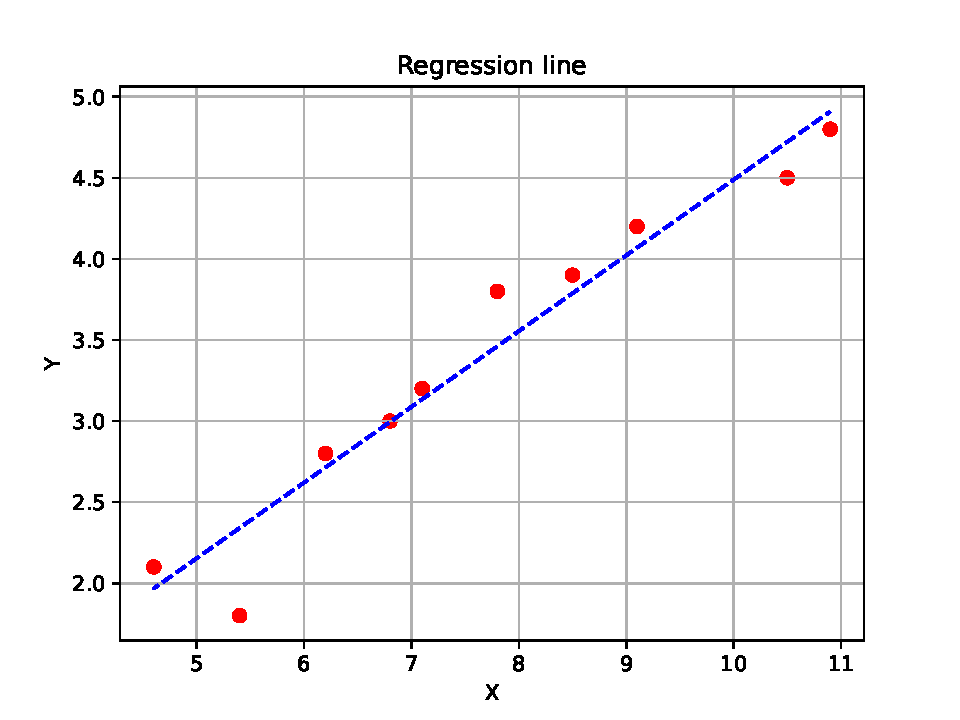
\includegraphics[width=0.8\textwidth]{regression_line.pdf}
    \caption{Графік лінійної регресії}
\end{figure}

\newpage

\section{Вправа 4. Кореляція Рангів Спірмана}

\begin{problem}
    Вивчається залежність між суб’єктивним відношенням співробітників фірми до
роботи (індексом задовільності роботою) та об’єктивним (текучості кадрів). Для 9
різних вікових груп приведені дані по деякому підприємству про індекси
задовільності роботою: $0.57; 0.38; 0.38; 0.24; 0.39; 0.59; 0.69; 0.77; 0.77$ та
відповідні дані про коефіцієнт текучості кадрів: $12.9; 12.9; 17.0; 37.1; 19.9;
7.9; 5.6; 6.1; 6.1$. Чим вище індекс задовільності, тим вище відповідний ранг.
Чим менший коефіцієнт текучості, тим вищий відповідний ранг. Обчислити
коефіцієнт кореляції рангів Спірмана між об’єктивним та суб’єктивним відношенням
співробітників підприємства до роботи, попередньо ранжувавши дані. Перевірити
статистичну значущість відповідного коефіцієнта кореляції.
\end{problem}

\textbf{Розв'язання.} Маємо дві ознаки: $X$ --- індекс задовільності роботою,
$Y$ --- коефіцієнт текучості кадрів з об'ємом вибірки $n=9$. Тепер, ранжуємо дані:
\begin{center}
    \begin{tabular}{|c|c|c|c|c|c|}
        \hline
        \textbf{Індекс задовільності $X$} & \textbf{Текучість кадрів $Y$} & \textbf{Ранг $R_X$} & \textbf{Ранг $R_Y$} & $d_i$ & $d_i^2$ \\
        \hline
        0.57 & 12.9 & 5 &   5.5 & -0.5 & 0.25 \\
        0.38 & 12.9 & 7.5 & 5.5 & 2.0 & 4.0 \\
        0.38 & 17.0 & 7.5 & 7 &   0.5 & 0.25 \\
        0.24 & 37.1 & 9 &   9 &   0.0 & 0.0 \\
        0.39 & 19.9 & 6 &   8 &  -2.0& 4.0 \\
        0.59 & 7.9 & 4 &    4 & 0.0 & 0.0 \\
        0.69 & 5.6 & 3 &    1 & 2.0 & 4.0 \\
        0.77 & 6.1 & 1.5 &  2.5 & -1.0 & 1.0 \\
        0.77 & 6.1 & 1.5 &  2.5 & -1.0 & 1.0 \\
        \hline
    \end{tabular}
\end{center}

В ознаці $X$ існує $m_X = 2$ пов'язаних об'єктів. Таким чином, згідно лекції,
рахуємо вираз $T_X = \frac{1}{12}\sum_{i=1}^{m_X}(t_{X,i}^3 - t_{X,i})$, де
$t_{X,i}$ --- число об'єктів у $i$-му пов'язаному рядку. В нашому випадку,
$t_{X,1} = t_{X,2} = 2$, тому маємо $T_X = 2\times
\frac{1}{12}\left(2^3-2\right)=1$.

Аналогічно, для $Y$ теж маємо $m_Y=2$ пов'язаних об'єктів з $t_{Y,1} = t_{Y,2} = 2$,
тому так само $T_Y = 1$. Тепер, обчислюємо коефіцієнт кореляції рангів Спірмана:
\begin{equation*}
    \overline{r}_C = \frac{n^3 - n - 6\sum_{i=1}^n d_i^2 - 6(T_X+T_Y)}{\sqrt{n^3-n-12T_X}\cdot \sqrt{n^3-n-12T_Y}}
    = \frac{9^3 - 9 - 6 \times 14.5 - 6(1+1)}{\sqrt{9^3-9-12} \cdot \sqrt{9^3-9-12}} \approx 0.877
\end{equation*}

Для перевірки статистичної значущості коефіцієнта кореляції, висунемо гіпотези:
\begin{itemize}
    \item $\mathcal{H}_0$: $r=0$.
    \item $\mathcal{H}_1$: $r\neq 0$.
\end{itemize}

Для цього, обчислюємо статистику $t=\overline{r}_C\sqrt{n-2}\Big/\sqrt{1-\overline{r}_C^2} \approx 4.83$. Задамо рівень 
значущості $q:=0.05$. За таблицями розподілу Стьюдента з $n-2=7$ ступенями свободи, маємо $t_{n-2,q} = t_{7,0.05} \approx 2.36$.
Оскільки $|t| > t_{n-2,q}$, то на рівні значущості $q=0.05$ відхиляємо гіпотезу $\mathcal{H}_0$ на користь гіпотези $\mathcal{H}_1$
про значущість коефіцієнта кореляції.

\newpage

\section{Вправа 5. Перевірка гіпотези про дисперсію}

\begin{problem}
    Дослідження, яке проводили протягом ряду років після того, як в практиці
    лижного спорту почала використовуватися тактика ковзанярського ходу, дають
    підставу припускати, що вона в умовах траси, яка спеціально підготовлена,
    забезпечує у чоловіків виграш в порівнянні з традиційною технікою в декілька
    хвилин. Нижче приведені дані, які одержано на змаганнях на дистанції 15 км
    для двох груп лижників: перші проходили дистанцію традиційним ходом, а другі
    – ковзанярським. Перша група лижників показала результати: $37.02; 36.74;
    37.82; 38.12; 36.91; 37.28; 38.21; 37.51; 37.5$, друга – наступні результати:
    $35.81; 35.61; 35.02; 35.53; 35.84; 35.12; 26.12; 36.49; 35.62$. Чи дозволяють
    ці результати стверджувати: що точності замірів часу проходження дистанцій в
    двох групах лижників однакові?
\end{problem}

\textbf{Розв'язання.} Під точністю замірів часу проходження дистанцій 
розуміємо однаковість дисперсій в двох групах. Вводимо дві гіпотези:
\begin{itemize}
    \item $\mathcal{H}_0$: $\sigma_X^2 = \sigma_Y^2$
    \item $\mathcal{H}_1$: $\sigma_X^2 \neq \sigma_Y^2$.
\end{itemize}

Об'єми двох вибірок однакові і дорівнюють $n=9$. Обчислюємо вибіркові середні:
\begin{equation*}
    \hat{\mu}_X = \frac{1}{n}\sum_{i=1}^n x_i \approx 37.457, \quad \hat{\mu}_Y = \frac{1}{n}\sum_{i=1}^n y_i \approx 34.573.
\end{equation*}

З них, обчислюємо вибіркові дисперсії:
\begin{equation*}
    \overline{\sigma}_X^2 = \frac{1}{n}\sum_{i=1}^n x_i^2 - \hat{\mu}_X^2 \approx 0.24, \quad \overline{\sigma}_Y^2 = \frac{1}{n}\sum_{i=1}^n y_i^2 - \hat{\mu}_Y^2 \approx 9.09.
\end{equation*}

А вже з них можемо обрахувати незміщенні оцінки дисперсій:
\begin{equation*}
    \hat{\sigma}_X^2 = \frac{n}{n-1}\overline{\sigma}_X^2 \approx 0.27, \quad \hat{\sigma}_Y^2 = \frac{n}{n-1}\overline{\sigma}_Y^2 \approx 10.23.
\end{equation*}

Таким чином, розглядаємо статистику $F=\hat{\sigma}_X^2/\hat{\sigma}_Y^2 \approx
0.026$. Введемо рівень значущості $q := 0.05$. Обраховуємо значення $F_1 :=
1/F_{n-1,n-1,q/2} = 1/F_{8,8,0.05} = 1/3.44 \approx 0.29$ та $F_2 :=
F_{n-1,n-1,q/2} = F_{8,8,0.05} \approx 3.44$. Оскільки $F \not\in (F_1,F_2)$, то 
на рівні значущості $q=0.1$ відхиляємо гіпотезу $\mathcal{H}_0$ на користь гіпотези
$\mathcal{H}_1$ про те, що дисперсії в двох групах неоднакові.

\end{document}